\documentclass{article}
\usepackage[utf8]{inputenc}
\usepackage[
    %backend=biber, 
    natbib=true,
    style=numeric,
    sorting=none
]{biblatex}
%\usepackage{biblatex} %Imports biblatex package
\addbibresource{literatura.bib} %Import the bibliography file
\usepackage[slovak]{babel}
\usepackage[T1]{fontenc}
\usepackage{amsmath}
\usepackage{fullpage}
\usepackage{graphicx}
\usepackage{txfonts}
\usepackage{gensymb}
\usepackage{eurosym}
\usepackage[export]{adjustbox}
\usepackage[symbol*]{footmisc}
\usepackage{mathtools}
\usepackage{enumitem}
\usepackage[unicode]{hyperref}
\usepackage{epsfig}
\usepackage{indentfirst}
\usepackage{subfig}
\usepackage{hyperref}
\usepackage{tabularx,ragged2e,booktabs,caption}
\usepackage{esvect}
\usepackage{pdfpages}
\usepackage{csquotes}
\usepackage{url}
\usepackage{textcomp}
\usepackage[hypcap = false]{caption}
\usepackage{calc}
\usepackage{graphicx}
\usepackage{color}
\usepackage{wrapfig}
\usepackage{float}
\usepackage{multirow}
\newfloat{graph}{htbp}{grp}
\floatname{graph}{Graf}
%\usepackage{fancyhdr}
%\usepackage[head=12pt]{geometry}

\title{P2_VIII}
\author{Ján Kovačovský}
\date{November 2019}

%\pagestyle{fancy}
%\lhead{Praktikum 2 - úloha 8}
%\rhead{Ján Kovačovský}


\begin{document}
\renewcommand{\thefootnote}{\arabic{footnote}}

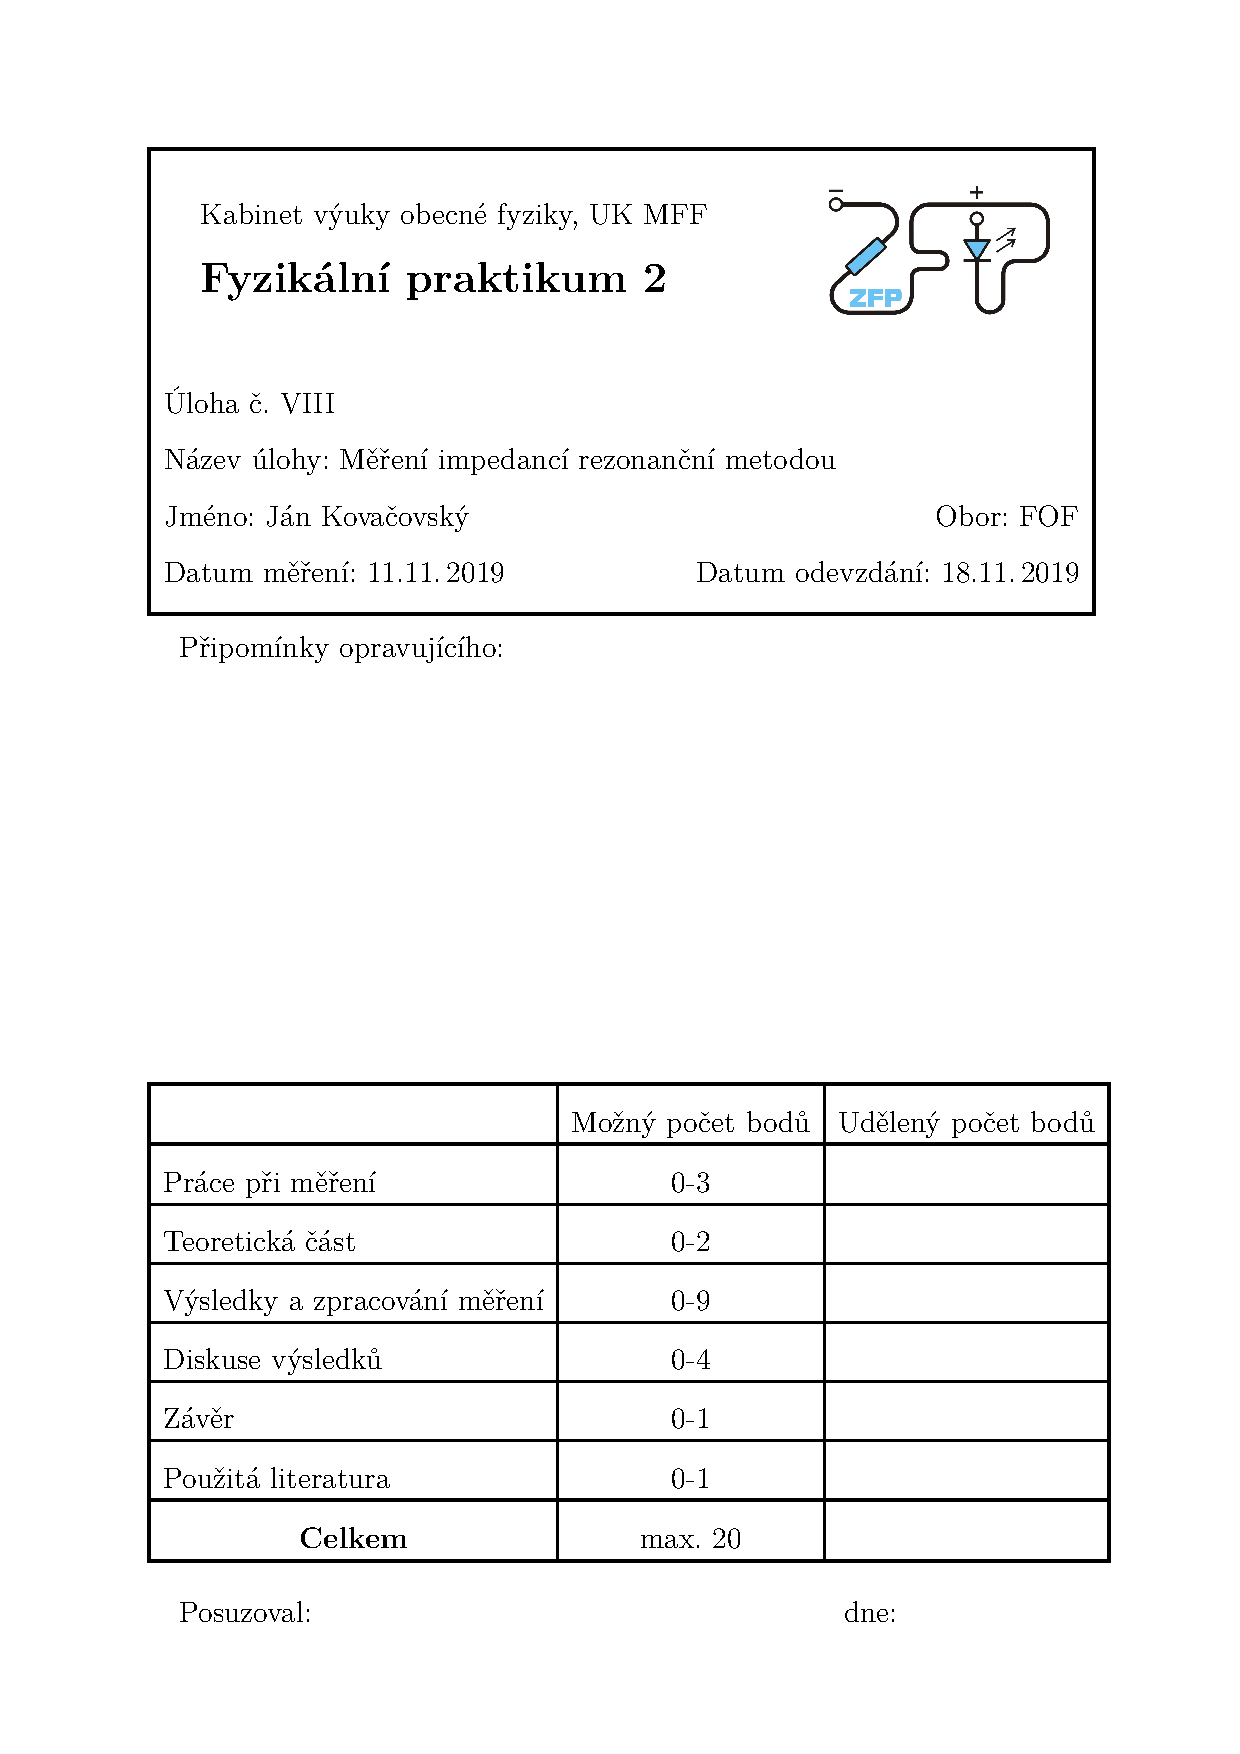
\includepdf[pages = 1]{titulka.pdf}

\section{Pracovná úloha}
\begin{enumerate}
    \item Zmerajte indukčnosti $L_A$ a $L_B$ a vlastné kapacity $C_A$ a $C_B$ cievok A a B.
    \item Z merania celkovej indukčnosti $L_{1,2}$ cievok A a B určite ich vzájomnú indukčnosť M. Diskutujte platnosť vzťahu medzi vzájomnou indukčnosťou M, indukčnosťami cievok $L_A$, $L_B$ a celkovou indukčnosťou $L_{1,2}$.
    \item Pre jedno zapojenie zmerajte rezonančnú krivku. Nameraný priebeh porovnajte graficky s teoretickým a vyhodnoťte mieru útlmu, činiteľ akosti a náhradný sériový odpor obvodu. 
    \item  Vykonajte kalibráciu otočného kondenzátora diferenčnou metódou a výsledok vyneste do grafu.
\end{enumerate}

\section{Teória}
\subsection{Rezonančná frekvencia RLC obvodu}
Pre $RLC$ obvod, ktorý je tvorený cievkou $L$, odporom $R$ a kapacitou $C$ zapojenými sériovo platí \cite{2}

\begin{equation}
    U = I\sqrt{R^2 + \left({\omega}L - \frac{1}{{\omega}C}\right)^2},
\end{equation}
kde $U$ je efektívne napätie, $I$ je efektívny prúd v obvode a $\omega$ je uhlová frekvencia striedavého prúdu. 

Pre paralelné zapojenie týchto prvkov platí obdobný vzťah 

\begin{equation}
    I = U\sqrt{\frac{1}{R^2} + \left({\omega}C - \frac{1}{{\omega}L}\right)^2}.
\end{equation}

Pri udržovaní konštantného napätia v sériovom obvode potečie obvodom maximálny prúd $I_r$ pri uhlovej frekvencii ${\omega}_r$, pre ktorú platí \cite{2}

\begin{equation}
    {\omega}_r = \frac{1}{\sqrt{LC}}. 
\end{equation}

Obdobne bude pre paralelný obvod platiť, že pri konštantnom prúde bude na prvkoch obvodu maximálne napätie $U_r$ znova pri uhlovej frekvencii ${\omega}_r$ vyhovujúcej vzťahu (3). Frekvenciu $f_r = {\omega}_r/2\pi$ nazývame rezonančná frekvencia. V sériovom obvode potom dochádza pri frekvencii $f_r$ k prúdovej rezonancii a v paralelnom k napäťovej.

Nakoľko ideálna cievka s nulovou vlastnou kapacitou $C_0$ neexistuje, upravíme vzťah (3) na 

\begin{equation}
    {\omega}_r = \frac{1}{\sqrt{L(C+C_0}}.
\end{equation}
\subsection{Redukovaná rezonančná krivka}
Redukovanou rezonančnou krivkou rozumieme závislosť premennej hodnoty prúdu $I/I_r$ = y pre sériový obvod, resp. napätia $U/U_r$ = y pre paralelný na rozdelení ${\omega}/{\omega}_r$ = x. Hodnoty $I_r$ a $U_r$, ku ktorým vzťahujeme prúd resp. napätie sú maximálne hodnoty týchto veličín pri rezonancii. Ak potom označíme 

\begin{equation}
    d = R\sqrt{\frac{C}{L}}
\end{equation}
pre sériový obvod a pre paralelný 

\begin{equation}
    d = \frac{1}{R}\sqrt{\frac{L}{C}}
\end{equation}
môžeme vzťahy (1) a (2) previesť na tvar 

\begin{equation}
    y^2 = \frac{d^2}{d^2 + \left(x-\frac{1}{x}\right)^2},
\end{equation}
ktorý popisuje redukovanú rezonančnú krivku. Veličinu $d$ nazývame mierou útlmu a charakterizuje šírku rezonančnej krivky. 

Činiteľ akosti $Q$ cievky je daný vzťahom podľa \cite{2}

\begin{equation}
    Q = \frac{{\omega}_rL}{R_S} = \frac{1}{d},
\end{equation}
kde $R_S$ je náhradný sériový odpor obvodu. 

\subsection{Indukčnosť a vlastná kapacita cievok}
Na rozdiel od ideálnej majú reálne cievky nenulovú vlastnú kapacitu $C_0$ pre ktorú platí \cite{2}

\begin{equation}
    \frac{1}{{\omega}_r^2} = L(C + C_0).
\end{equation}

Meraním rezonančnej frekvencie pre rôzne hodnoty premennej kapacity určíme hodnoty $C_0$ a $L$ a ich štatistické chyby lineárnou regresiou. 
\subsection{Vzájomná indukčnosť cievok}
Celková indukčnosť sériovo zapojených cievok $L_A$ a $L_B$ je daná \cite{2}

\begin{equation}
    L_{1,2} = L_A + L_B \pm 2M,
\end{equation}
kde $M$ označuje vzájomnú indukčnosť týchto cievok, pre ktoré platí \cite{2}

\begin{equation}
    M = \frac{L_1-L_2}{4}.
\end{equation}
Kladné znamienko, resp. záporné označuje súhlasný, resp. nesúhlasný smer vinutia. 

\subsection{Kalibrácia otočného kondenzátora}
Kapacitu kondenzátora určíme diferenčnou metódou. Obvod s kondenzátorom so známou kapacitou $C_1$ vyladíme do rezonancie. Následne k nemu paralelne pripojíme kondenzátor s neznámou kapacitou, vyladíme obvod do rezonancie a odpočítame kapacitu $C_2$. Neznámu kapacitu $C_x$ určíme zo vzťahu podľa \cite{2}

\begin{equation}
    C_x = C_1 - C_2.
\end{equation}

\subsection{Spracovanie merania}
Chyby merania počítame podľa \cite{1} ako
    \begin{equation}
        \sigma_v = \sqrt{\sigma_{\text{stat}}^2 + \sigma_{\text{mer}}^2 }
    \end{equation}
    kde $\sigma_{\text{stat}}$ je štatistická chyba a $\sigma_{\text{mer}}$ je chyba meradla (polovica dieliku na stupnici) pri meraní veličiny $v$. 
    
Pri výpočte chýb odvodených veličín používame Gaussov vzorec podľa \cite{1}
    \begin{equation}
            \sigma_f = \sqrt{\sum_{i=1}^{n}\left( \frac{\partial f}{\partial x_i}\right)^2 \sigma_{x_i}^2}.
    \end{equation}
kde $x_i$ sú namerané veličiny v jednotlivých meraniach $i$, $n$ je ich počet a $\sigma$ je ich rozptyl, dopočítame ostávajúce chyby.

Pri digitálnych prístrojoch počítame chybu spôsobom uvedeným v návode.
\newpage


\subsection{Schéma zapojenia obvodu}

\begin{figure}[!htbp]
		\centering
		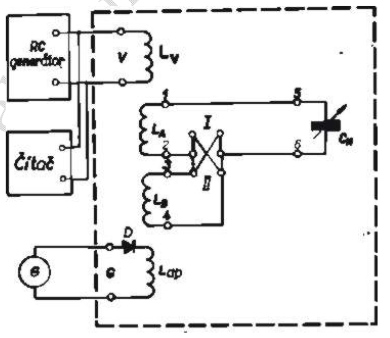
\includegraphics[height = 6cm]{rezobvod.PNG}
		\caption{Schéma zapojenia rezonančného obvodu. Prevzaté z \cite{2}.}
		\label{fig3:bandf} 
	\end{figure}

\section{Výsledky merania}
\subsection{Vlastná kapacita a indukčnosť cievok}
Meranie u oboch cievok sme opakovali pre 5 hodnôt danej kapacity $C$ kondenzátora. Rezonančnú frekvenciu sme neurčovali priamo, nakoľko priebeh rezonančnej funkcie v okolí maxima je príliš konštantný a galvanometrom, s ktorým sme merali, nedokážeme určiť presnú hodnotu maxima. Našli sme preto dve frekvencie $f_1$ a $f_2$, pre ktoré galvanometer ukazoval rovnakú výchylku, t.j. symetrické hodnoty $f_1$, $f_2$ z oboch strán rezonančnej krivky. Hodnotu maxima potom dostaneme ako aritmetický priemer týchto dvoch hodnôt. Namerané hodnoty a dopočítané veličiny sú uvedené v tabuľke 1. Chybu merania rezonančnej frekvencie odhadujeme na 1 kHz a pre kapacitu kondenzátora na 0.2 pF.

\begin{table}[!htbp]
\centering
\captionof{table}{Závislosť rezonančnej frekvencie na kapacite pre cievku A}
\label{tab:cvA}
\begin{tabular}{|l|l|l|l|l|}
\hline
$C$ [pF] & $f_1$ [kHz] & $f_2$ [kHz] &   $f_r$ [kHz]    &   $1/\omega_r^2$ [10$^{-14}$s$^2$]   \\ \hline
200     & 674.6   & 680.0   & 677.3 & 5.5  \\ \hline
400     & 508.4   & 510.3   & 509.4 & 9.8  \\ \hline
600     & 420.9   & 425.4   & 423.2 & 14.1 \\ \hline
800     & 368.0   & 373.0   & 370.5 & 18.5 \\ \hline
1000    & 332.1   & 336.3   & 334.2 & 22.7 \\ \hline
\end{tabular}
\end{table}

\begin{table}[!htbp]
\captionof{table}{Závislosť rezonančnej frekvencie na kapacite pre cievku B}
\label{tab:cvB}
\centering
\begin{tabular}{|l|l|l|l|l|}
\hline
$C$ [pF] & $f_1$ [kHz] & $f_2$ [kHz] &   $f_r$ [kHz]    &   $1/\omega_r^2$ [10$^{-14}$s$^2$]   \\ \hline
1000    & 313.4   & 322.6   & 318.0 & 25.0 \\ \hline
800     & 349.0   & 359.9   & 354.5 & 20.2 \\ \hline
600     & 400.7   & 414.1   & 407.4 & 15.3 \\ \hline
400     & 486.5   & 502.8   & 494.7 & 10.4 \\ \hline
200     & 676.8   & 689.8   & 683.3 & 5.4  \\ \hline
\end{tabular}
\end{table}

\newpage
Hodnoty z tabuliek \ref{tab:cvA} a \ref{tab:cvB} sú vynesené do grafu \ref{graf:cievkaAB}, kde sú preložené lineárnymi funkciami tvaru $f(x) = a{\cdot}(x+b)$ podľa vzťahu (9). Výsledky tohoto fitu sú zhrnuté v nasledujúcej tabuľke, t.j. tab. 3, kde chyba indukčnosti $L$ a kapacity $C$ je určená podľa vzťahu (13) ako súčet chyby fitu a chyby vypočítanej vzťahom podľa (14)

\begin{equation} \label{eq:cvchyba}
    \sigma_L = \sigma_{C_0} = \sqrt{\frac{1}{n-1}\sum_i \left[ \left(2\frac{\sigma_f}{f_i} \right)^2 + \left(\frac{\sigma_C}{C_i} \right)^2 \right]}
\end{equation}

\begin{graph}[H]
		\centering
		% GNUPLOT: LaTeX picture with Postscript
\begingroup
  \makeatletter
  \providecommand\color[2][]{%
    \GenericError{(gnuplot) \space\space\space\@spaces}{%
      Package color not loaded in conjunction with
      terminal option `colourtext'%
    }{See the gnuplot documentation for explanation.%
    }{Either use 'blacktext' in gnuplot or load the package
      color.sty in LaTeX.}%
    \renewcommand\color[2][]{}%
  }%
  \providecommand\includegraphics[2][]{%
    \GenericError{(gnuplot) \space\space\space\@spaces}{%
      Package graphicx or graphics not loaded%
    }{See the gnuplot documentation for explanation.%
    }{The gnuplot epslatex terminal needs graphicx.sty or graphics.sty.}%
    \renewcommand\includegraphics[2][]{}%
  }%
  \providecommand\rotatebox[2]{#2}%
  \@ifundefined{ifGPcolor}{%
    \newif\ifGPcolor
    \GPcolorfalse
  }{}%
  \@ifundefined{ifGPblacktext}{%
    \newif\ifGPblacktext
    \GPblacktexttrue
  }{}%
  % define a \g@addto@macro without @ in the name:
  \let\gplgaddtomacro\g@addto@macro
  % define empty templates for all commands taking text:
  \gdef\gplbacktext{}%
  \gdef\gplfronttext{}%
  \makeatother
  \ifGPblacktext
    % no textcolor at all
    \def\colorrgb#1{}%
    \def\colorgray#1{}%
  \else
    % gray or color?
    \ifGPcolor
      \def\colorrgb#1{\color[rgb]{#1}}%
      \def\colorgray#1{\color[gray]{#1}}%
      \expandafter\def\csname LTw\endcsname{\color{white}}%
      \expandafter\def\csname LTb\endcsname{\color{black}}%
      \expandafter\def\csname LTa\endcsname{\color{black}}%
      \expandafter\def\csname LT0\endcsname{\color[rgb]{1,0,0}}%
      \expandafter\def\csname LT1\endcsname{\color[rgb]{0,1,0}}%
      \expandafter\def\csname LT2\endcsname{\color[rgb]{0,0,1}}%
      \expandafter\def\csname LT3\endcsname{\color[rgb]{1,0,1}}%
      \expandafter\def\csname LT4\endcsname{\color[rgb]{0,1,1}}%
      \expandafter\def\csname LT5\endcsname{\color[rgb]{1,1,0}}%
      \expandafter\def\csname LT6\endcsname{\color[rgb]{0,0,0}}%
      \expandafter\def\csname LT7\endcsname{\color[rgb]{1,0.3,0}}%
      \expandafter\def\csname LT8\endcsname{\color[rgb]{0.5,0.5,0.5}}%
    \else
      % gray
      \def\colorrgb#1{\color{black}}%
      \def\colorgray#1{\color[gray]{#1}}%
      \expandafter\def\csname LTw\endcsname{\color{white}}%
      \expandafter\def\csname LTb\endcsname{\color{black}}%
      \expandafter\def\csname LTa\endcsname{\color{black}}%
      \expandafter\def\csname LT0\endcsname{\color{black}}%
      \expandafter\def\csname LT1\endcsname{\color{black}}%
      \expandafter\def\csname LT2\endcsname{\color{black}}%
      \expandafter\def\csname LT3\endcsname{\color{black}}%
      \expandafter\def\csname LT4\endcsname{\color{black}}%
      \expandafter\def\csname LT5\endcsname{\color{black}}%
      \expandafter\def\csname LT6\endcsname{\color{black}}%
      \expandafter\def\csname LT7\endcsname{\color{black}}%
      \expandafter\def\csname LT8\endcsname{\color{black}}%
    \fi
  \fi
    \setlength{\unitlength}{0.0500bp}%
    \ifx\gptboxheight\undefined%
      \newlength{\gptboxheight}%
      \newlength{\gptboxwidth}%
      \newsavebox{\gptboxtext}%
    \fi%
    \setlength{\fboxrule}{0.5pt}%
    \setlength{\fboxsep}{1pt}%
\begin{picture}(9070.00,5668.00)%
    \gplgaddtomacro\gplbacktext{%
      \csname LTb\endcsname%%
      \put(682,1178){\makebox(0,0)[r]{\strut{}$5$}}%
      \csname LTb\endcsname%%
      \put(682,2127){\makebox(0,0)[r]{\strut{}$10$}}%
      \csname LTb\endcsname%%
      \put(682,3076){\makebox(0,0)[r]{\strut{}$15$}}%
      \csname LTb\endcsname%%
      \put(682,4024){\makebox(0,0)[r]{\strut{}$20$}}%
      \csname LTb\endcsname%%
      \put(682,4973){\makebox(0,0)[r]{\strut{}$25$}}%
      \csname LTb\endcsname%%
      \put(1251,484){\makebox(0,0){\strut{}$200$}}%
      \csname LTb\endcsname%%
      \put(2124,484){\makebox(0,0){\strut{}$300$}}%
      \csname LTb\endcsname%%
      \put(2997,484){\makebox(0,0){\strut{}$400$}}%
      \csname LTb\endcsname%%
      \put(3870,484){\makebox(0,0){\strut{}$500$}}%
      \csname LTb\endcsname%%
      \put(4744,484){\makebox(0,0){\strut{}$600$}}%
      \csname LTb\endcsname%%
      \put(5617,484){\makebox(0,0){\strut{}$700$}}%
      \csname LTb\endcsname%%
      \put(6490,484){\makebox(0,0){\strut{}$800$}}%
      \csname LTb\endcsname%%
      \put(7363,484){\makebox(0,0){\strut{}$900$}}%
      \csname LTb\endcsname%%
      \put(8236,484){\makebox(0,0){\strut{}$1000$}}%
    }%
    \gplgaddtomacro\gplfronttext{%
      \csname LTb\endcsname%%
      \put(198,3075){\rotatebox{-270}{\makebox(0,0){\strut{}$1/\omega_r^2$ [10$^-{14}$s$^2$]}}}%
      \put(4743,154){\makebox(0,0){\strut{}$C$ [pF]}}%
      \csname LTb\endcsname%%
      \put(4246,5274){\makebox(0,0)[r]{\strut{}$f_A(C) = 0.02150{\cdot}(C+56.3)$}}%
      \csname LTb\endcsname%%
      \put(4246,5054){\makebox(0,0)[r]{\strut{}$f_B(C) = 0.02453{\cdot}(C+21.7)$}}%
      \csname LTb\endcsname%%
      \put(4246,4834){\makebox(0,0)[r]{\strut{}Cievka A}}%
      \csname LTb\endcsname%%
      \put(4246,4614){\makebox(0,0)[r]{\strut{}Cievka B}}%
    }%
    \gplbacktext
    \put(0,0){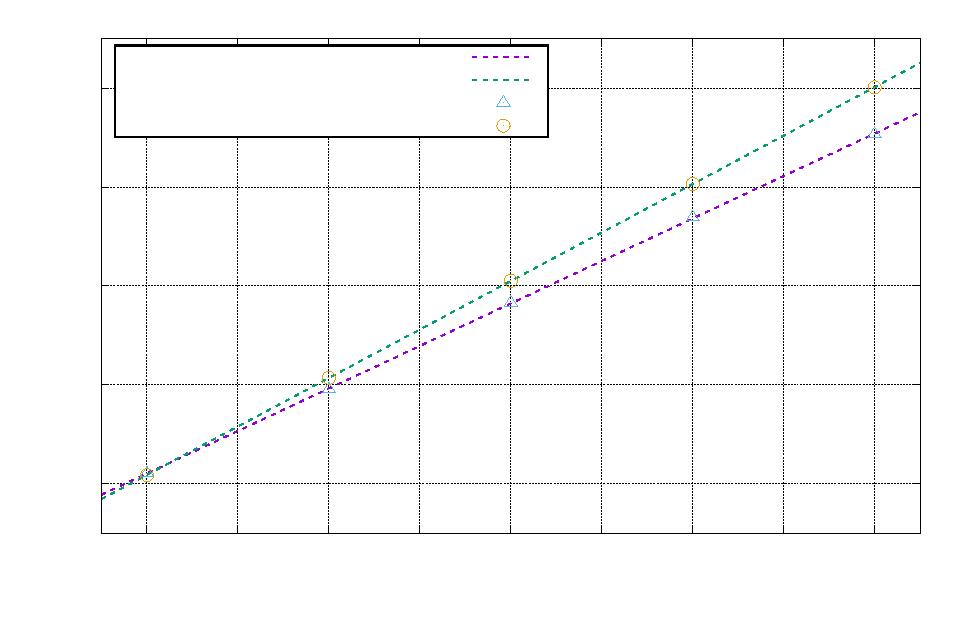
\includegraphics{cievkaAB}}%
    \gplfronttext
  \end{picture}%
\endgroup

		\caption{Závislosť prevrátenej hodnoty druhej mocniny uhlovej frekvencie na kapacite $C$ pre jednotlivé cievky}
		\label{graf:cievkaAB}
\end{graph}

\begin{table}[!htbp]
\captionof{table}{Výsledné hodnoty indukčností a vlastných kapacít cievok A a B}
\centering
\begin{tabular}{|l|l|l|}
\hline
 cievka & $C_0$ [pF] & $L$ [$\mu$H] \\ \hline
 A   & 56.3 $\pm$  0.8  & 215.0 $\pm$ 1.6   \\ \hline
 B   & 21.7 $\pm$ 1.1   & 245.3 $\pm$ 0.7    \\ \hline

\end{tabular}
\end{table}

\subsection{Vzájomná indukčnosť cievok}
Postup merania bol obdobný ako v prvej úlohe. Tu nám už ale pôsobí aj vzájomná indukčnosť týchto cievok a teda nemožno použiť vypočítané hodnoty z predošlej úlohy. Meranie sme vykonali znova pre 5 hodnôt, jednak pri súhlasnom a potom nesúhlasnom vinutí \footnote{používame vzorec (10), v ktorom $+$ značí súhlasný smer vinutia oboch cievok a $-$ nesúhlasný}. V tabuľke \ref{tab:cvAB} sú uvedené namerané hodnoty pri súhlasnom vinutí zapojenia cievok a v tab. \ref{tab:cvBA} pri nesúhlasnom. 

Chyba merania vzájomnej indukčnosti bola určená vzťahom (13) ako súčet chyby fitu a prenosu chyby vypočítanej vzťahom pre prenos chyby podľa (14)

\begin{equation}
    \sigma_M = M \sqrt{\left(\frac{\sigma_{L_1}}{L_1}\right)^2 + \left(\frac{\sigma_{L_2}}{L_2}\right)^2}
\end{equation}

\begin{table}[!htbp]
\captionof{table}{Závislosť rezonančnej frekvencie na kapacite pre zapojenie cievok pri súhlasnom smere vinutia}
\label{tab:cvAB}
\centering
\begin{tabular}{|l|l|l|l|l|}
\hline
$C$ [pF] & $f_1$ [kHz] & $f_2$ [kHz] &   $f_r$ [kHz]    &   $1/\omega_r^2$ [10$^{-14}$s$^2$]   \\ \hline
200     & 430.0   & 461.3   & 445.7 & 12.8 \\ \hline
400     & 312.5   & 334.5   & 323.5 & 24.2 \\ \hline
600     & 256.3   & 276.3   & 266.3 & 35.7 \\ \hline
800     & 222.6   & 241.0   & 231.8 & 47.1 \\ \hline
1000    & 199.8   & 216.3   & 208.1 & 58.5 \\ \hline
\end{tabular}
\end{table}

\begin{table}[!htbp]
\captionof{table}{Závislosť rezonančnej frekvencie na kapacite pre zapojenie cievok pri nesúhlasnom smere vinutia}
\label{tab:cvBA}
\centering
\begin{tabular}{|l|l|l|l|l|}
\hline
$C$ [pF] & $f_1$ [kHz] & $f_2$ [kHz] &   $f_r$ [kHz]    &   $1/\omega_r^2$ [10$^{-14}$s$^2$]   \\ \hline
1000    & 266.8   & 275.3   & 271.1 & 34.5 \\ \hline
800     & 296.9   & 306.9   & 301.9 & 27.8 \\ \hline
600     & 342.5   & 351.7   & 347.1 & 21.0 \\ \hline
400     & 417.5   & 424.1   & 420.8 & 14.3 \\ \hline
200     & 573.6   & 584.8   & 579.2 & 7.6  \\ \hline
\end{tabular}
\end{table}

Hodnoty z tabuliek \ref{tab:cvAB} a \ref{tab:cvBA} sú vynesené do grafu \ref{graf:ABvinutie}, kde sú preložené lineárnymi funkciami tvaru $f(x) = a{\cdot}(x+b)$ podľa vzťahu (9). Chyba indukčnosti $L$ a kapacity $C$ je určená podľa vzťahu (15).

\begin{graph}[H]
		\centering
		% GNUPLOT: LaTeX picture with Postscript
\begingroup
  \makeatletter
  \providecommand\color[2][]{%
    \GenericError{(gnuplot) \space\space\space\@spaces}{%
      Package color not loaded in conjunction with
      terminal option `colourtext'%
    }{See the gnuplot documentation for explanation.%
    }{Either use 'blacktext' in gnuplot or load the package
      color.sty in LaTeX.}%
    \renewcommand\color[2][]{}%
  }%
  \providecommand\includegraphics[2][]{%
    \GenericError{(gnuplot) \space\space\space\@spaces}{%
      Package graphicx or graphics not loaded%
    }{See the gnuplot documentation for explanation.%
    }{The gnuplot epslatex terminal needs graphicx.sty or graphics.sty.}%
    \renewcommand\includegraphics[2][]{}%
  }%
  \providecommand\rotatebox[2]{#2}%
  \@ifundefined{ifGPcolor}{%
    \newif\ifGPcolor
    \GPcolorfalse
  }{}%
  \@ifundefined{ifGPblacktext}{%
    \newif\ifGPblacktext
    \GPblacktexttrue
  }{}%
  % define a \g@addto@macro without @ in the name:
  \let\gplgaddtomacro\g@addto@macro
  % define empty templates for all commands taking text:
  \gdef\gplbacktext{}%
  \gdef\gplfronttext{}%
  \makeatother
  \ifGPblacktext
    % no textcolor at all
    \def\colorrgb#1{}%
    \def\colorgray#1{}%
  \else
    % gray or color?
    \ifGPcolor
      \def\colorrgb#1{\color[rgb]{#1}}%
      \def\colorgray#1{\color[gray]{#1}}%
      \expandafter\def\csname LTw\endcsname{\color{white}}%
      \expandafter\def\csname LTb\endcsname{\color{black}}%
      \expandafter\def\csname LTa\endcsname{\color{black}}%
      \expandafter\def\csname LT0\endcsname{\color[rgb]{1,0,0}}%
      \expandafter\def\csname LT1\endcsname{\color[rgb]{0,1,0}}%
      \expandafter\def\csname LT2\endcsname{\color[rgb]{0,0,1}}%
      \expandafter\def\csname LT3\endcsname{\color[rgb]{1,0,1}}%
      \expandafter\def\csname LT4\endcsname{\color[rgb]{0,1,1}}%
      \expandafter\def\csname LT5\endcsname{\color[rgb]{1,1,0}}%
      \expandafter\def\csname LT6\endcsname{\color[rgb]{0,0,0}}%
      \expandafter\def\csname LT7\endcsname{\color[rgb]{1,0.3,0}}%
      \expandafter\def\csname LT8\endcsname{\color[rgb]{0.5,0.5,0.5}}%
    \else
      % gray
      \def\colorrgb#1{\color{black}}%
      \def\colorgray#1{\color[gray]{#1}}%
      \expandafter\def\csname LTw\endcsname{\color{white}}%
      \expandafter\def\csname LTb\endcsname{\color{black}}%
      \expandafter\def\csname LTa\endcsname{\color{black}}%
      \expandafter\def\csname LT0\endcsname{\color{black}}%
      \expandafter\def\csname LT1\endcsname{\color{black}}%
      \expandafter\def\csname LT2\endcsname{\color{black}}%
      \expandafter\def\csname LT3\endcsname{\color{black}}%
      \expandafter\def\csname LT4\endcsname{\color{black}}%
      \expandafter\def\csname LT5\endcsname{\color{black}}%
      \expandafter\def\csname LT6\endcsname{\color{black}}%
      \expandafter\def\csname LT7\endcsname{\color{black}}%
      \expandafter\def\csname LT8\endcsname{\color{black}}%
    \fi
  \fi
    \setlength{\unitlength}{0.0500bp}%
    \ifx\gptboxheight\undefined%
      \newlength{\gptboxheight}%
      \newlength{\gptboxwidth}%
      \newsavebox{\gptboxtext}%
    \fi%
    \setlength{\fboxrule}{0.5pt}%
    \setlength{\fboxsep}{1pt}%
\begin{picture}(9070.00,5668.00)%
    \gplgaddtomacro\gplbacktext{%
      \csname LTb\endcsname%%
      \put(682,1113){\makebox(0,0)[r]{\strut{}$10$}}%
      \csname LTb\endcsname%%
      \put(682,1931){\makebox(0,0)[r]{\strut{}$20$}}%
      \csname LTb\endcsname%%
      \put(682,2748){\makebox(0,0)[r]{\strut{}$30$}}%
      \csname LTb\endcsname%%
      \put(682,3566){\makebox(0,0)[r]{\strut{}$40$}}%
      \csname LTb\endcsname%%
      \put(682,4384){\makebox(0,0)[r]{\strut{}$50$}}%
      \csname LTb\endcsname%%
      \put(682,5202){\makebox(0,0)[r]{\strut{}$60$}}%
      \csname LTb\endcsname%%
      \put(1251,484){\makebox(0,0){\strut{}$200$}}%
      \csname LTb\endcsname%%
      \put(2124,484){\makebox(0,0){\strut{}$300$}}%
      \csname LTb\endcsname%%
      \put(2997,484){\makebox(0,0){\strut{}$400$}}%
      \csname LTb\endcsname%%
      \put(3870,484){\makebox(0,0){\strut{}$500$}}%
      \csname LTb\endcsname%%
      \put(4744,484){\makebox(0,0){\strut{}$600$}}%
      \csname LTb\endcsname%%
      \put(5617,484){\makebox(0,0){\strut{}$700$}}%
      \csname LTb\endcsname%%
      \put(6490,484){\makebox(0,0){\strut{}$800$}}%
      \csname LTb\endcsname%%
      \put(7363,484){\makebox(0,0){\strut{}$900$}}%
      \csname LTb\endcsname%%
      \put(8236,484){\makebox(0,0){\strut{}$1000$}}%
    }%
    \gplgaddtomacro\gplfronttext{%
      \csname LTb\endcsname%%
      \put(198,3075){\rotatebox{-270}{\makebox(0,0){\strut{}$1/\omega_r^2$ [10$^-{14}$s$^2$]}}}%
      \put(4743,154){\makebox(0,0){\strut{}$C$ [pF]}}%
      \csname LTb\endcsname%%
      \put(4246,5274){\makebox(0,0)[r]{\strut{}$f_{+}(C) = 0.05715{\cdot}(C+23.9)$}}%
      \csname LTb\endcsname%%
      \put(4246,5054){\makebox(0,0)[r]{\strut{}$f_{-}(C) = 0.03365{\cdot}(C+25.3)$}}%
      \csname LTb\endcsname%%
      \put(4246,4834){\makebox(0,0)[r]{\strut{}Súhlasné vinutie (+)}}%
      \csname LTb\endcsname%%
      \put(4246,4614){\makebox(0,0)[r]{\strut{}Nesúhlasné vinutie (-)}}%
    }%
    \gplbacktext
    \put(0,0){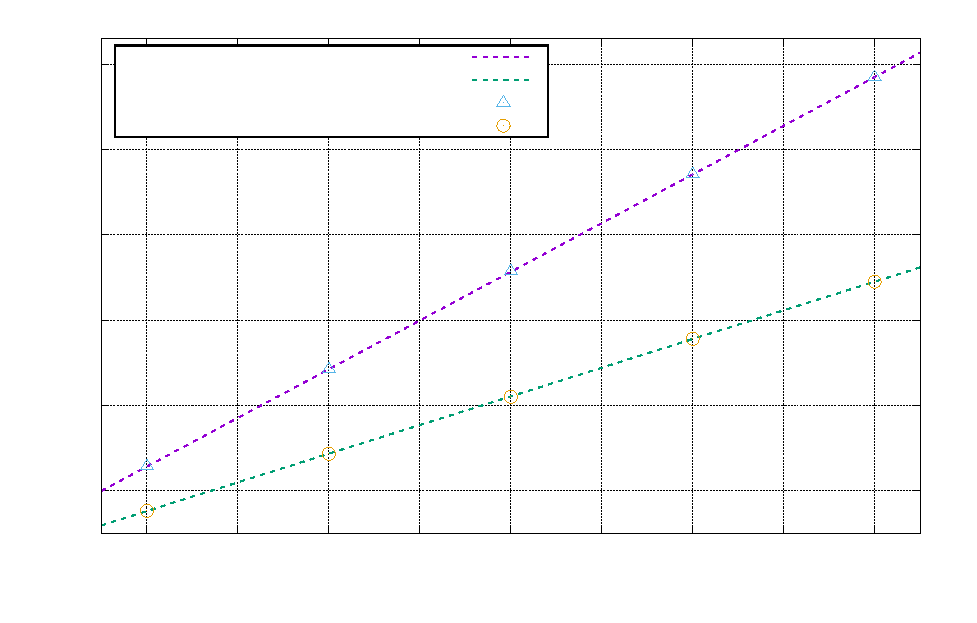
\includegraphics{ABvinutie}}%
    \gplfronttext
  \end{picture}%
\endgroup

		\caption{Závislosť prevrátenej hodnoty druhej mocniny uhlovej frekvencie na kapacite $C$ pre obe smery vinutia cievok}
		\label{graf:ABvinutie}
\end{graph}

Z oboch fitov potom dostávame indukčnosti pre oba smery vinutia ako
$$ \text{$L_+$ = (571.5 $\pm$ 7.8) $\mu$H, $L_-$ = (336.5 $\pm$ 7.2) $\mu$H}$$
a použitím vzťahu (11) aj vzájomnú indukčnosť použitých cievok
$$\text{$M$ = (58.8 $\pm$ 3.3) 
$\mu$H}. $$

Vzťahom (10) následne dopočítame hodnoty celkovej indukčnosti pre obe smery zapojenia vinutia a tak ich môžeme porovnať s vyššie vypočítanými. Tieto hodnoty nám vyšli ako

$$\text{$L^{'}_+$ = (577.9 $\pm$ 9.2) $\mu$H a $L^{'}_-$ = (342.7 $\pm$ 8.9) $\mu$H.} $$

Hodnoty sa teda v rámci chyby zhodujú a môžeme považovať vzťah (10) resp. (11) za potvrdený.


\newpage
\subsection{Rezonančná krivka}
Namerali sme rezonančnú krivku pre nesúhlasne vinutie cievok A,B a hodnotu $C$ = 200 pF. Maximálna výchylka na galvanometri bola 47, čo zodpovedá hodnote $y^2 = 1$ a $x = f/f_r$ na redukovanej rezonančnej krivke. Nakoľko pracujeme s rovnakým zapojením obvodu ako v predošlej úlohe, t.j. nesúhlasné vinutie cievok A,B pre kapacitu $C=200 pF$, môžeme použiť hodnotu $f_r = (579.2 \pm 1.1)$ kHz odtiaľ.

\begin{table}[!htbp]
\captionof{table}{Namerané hodnoty výchyliek na galvanometri v závislosti na frekvencii}
\centering
\begin{tabular}{|l|l|l|l|l|l|l|l|}
\hline
dieliky & $f$ [kHz] & x & $y^2$ & dieliky & $f$ [kHz] & x & $y^2$ \\ \hline
47 & 578.5 & 0.9988 & 1.0000 & 35 & 585.4 & 1.0107 & 0.7447 \\  \hline
45 & 575.8 & 0.9941 & 0.9574 & 30 & 587.8 & 1.0148 & 0.6383 \\  \hline
40 & 573.5 & 0.9902 & 0.8511 & 25 & 590.6 & 1.0197 & 0.5319 \\  \hline
30 & 569.9 & 0.9839 & 0.6383 & 20 & 594.3 & 1.0261 & 0.4255 \\  \hline
25 & 567.8 & 0.9803 & 0.5319 & 15 & 599.9 & 1.0357 & 0.3191 \\  \hline
20 & 565.6 & 0.9765 & 0.4255 & 10 & 610   & 1.0532 & 0.2128 \\ \hline
\end{tabular}
\end{table}

\begin{graph}[ht]
		\centering
		% GNUPLOT: LaTeX picture with Postscript
\begingroup
  \makeatletter
  \providecommand\color[2][]{%
    \GenericError{(gnuplot) \space\space\space\@spaces}{%
      Package color not loaded in conjunction with
      terminal option `colourtext'%
    }{See the gnuplot documentation for explanation.%
    }{Either use 'blacktext' in gnuplot or load the package
      color.sty in LaTeX.}%
    \renewcommand\color[2][]{}%
  }%
  \providecommand\includegraphics[2][]{%
    \GenericError{(gnuplot) \space\space\space\@spaces}{%
      Package graphicx or graphics not loaded%
    }{See the gnuplot documentation for explanation.%
    }{The gnuplot epslatex terminal needs graphicx.sty or graphics.sty.}%
    \renewcommand\includegraphics[2][]{}%
  }%
  \providecommand\rotatebox[2]{#2}%
  \@ifundefined{ifGPcolor}{%
    \newif\ifGPcolor
    \GPcolorfalse
  }{}%
  \@ifundefined{ifGPblacktext}{%
    \newif\ifGPblacktext
    \GPblacktexttrue
  }{}%
  % define a \g@addto@macro without @ in the name:
  \let\gplgaddtomacro\g@addto@macro
  % define empty templates for all commands taking text:
  \gdef\gplbacktext{}%
  \gdef\gplfronttext{}%
  \makeatother
  \ifGPblacktext
    % no textcolor at all
    \def\colorrgb#1{}%
    \def\colorgray#1{}%
  \else
    % gray or color?
    \ifGPcolor
      \def\colorrgb#1{\color[rgb]{#1}}%
      \def\colorgray#1{\color[gray]{#1}}%
      \expandafter\def\csname LTw\endcsname{\color{white}}%
      \expandafter\def\csname LTb\endcsname{\color{black}}%
      \expandafter\def\csname LTa\endcsname{\color{black}}%
      \expandafter\def\csname LT0\endcsname{\color[rgb]{1,0,0}}%
      \expandafter\def\csname LT1\endcsname{\color[rgb]{0,1,0}}%
      \expandafter\def\csname LT2\endcsname{\color[rgb]{0,0,1}}%
      \expandafter\def\csname LT3\endcsname{\color[rgb]{1,0,1}}%
      \expandafter\def\csname LT4\endcsname{\color[rgb]{0,1,1}}%
      \expandafter\def\csname LT5\endcsname{\color[rgb]{1,1,0}}%
      \expandafter\def\csname LT6\endcsname{\color[rgb]{0,0,0}}%
      \expandafter\def\csname LT7\endcsname{\color[rgb]{1,0.3,0}}%
      \expandafter\def\csname LT8\endcsname{\color[rgb]{0.5,0.5,0.5}}%
    \else
      % gray
      \def\colorrgb#1{\color{black}}%
      \def\colorgray#1{\color[gray]{#1}}%
      \expandafter\def\csname LTw\endcsname{\color{white}}%
      \expandafter\def\csname LTb\endcsname{\color{black}}%
      \expandafter\def\csname LTa\endcsname{\color{black}}%
      \expandafter\def\csname LT0\endcsname{\color{black}}%
      \expandafter\def\csname LT1\endcsname{\color{black}}%
      \expandafter\def\csname LT2\endcsname{\color{black}}%
      \expandafter\def\csname LT3\endcsname{\color{black}}%
      \expandafter\def\csname LT4\endcsname{\color{black}}%
      \expandafter\def\csname LT5\endcsname{\color{black}}%
      \expandafter\def\csname LT6\endcsname{\color{black}}%
      \expandafter\def\csname LT7\endcsname{\color{black}}%
      \expandafter\def\csname LT8\endcsname{\color{black}}%
    \fi
  \fi
    \setlength{\unitlength}{0.0500bp}%
    \ifx\gptboxheight\undefined%
      \newlength{\gptboxheight}%
      \newlength{\gptboxwidth}%
      \newsavebox{\gptboxtext}%
    \fi%
    \setlength{\fboxrule}{0.5pt}%
    \setlength{\fboxsep}{1pt}%
\begin{picture}(9070.00,5102.00)%
    \gplgaddtomacro\gplbacktext{%
      \csname LTb\endcsname%%
      \put(814,1052){\makebox(0,0)[r]{\strut{}$0$}}%
      \csname LTb\endcsname%%
      \put(814,1748){\makebox(0,0)[r]{\strut{}$0.2$}}%
      \csname LTb\endcsname%%
      \put(814,2444){\makebox(0,0)[r]{\strut{}$0.4$}}%
      \csname LTb\endcsname%%
      \put(814,3141){\makebox(0,0)[r]{\strut{}$0.6$}}%
      \csname LTb\endcsname%%
      \put(814,3837){\makebox(0,0)[r]{\strut{}$0.8$}}%
      \csname LTb\endcsname%%
      \put(814,4533){\makebox(0,0)[r]{\strut{}$1$}}%
      \csname LTb\endcsname%%
      \put(946,484){\makebox(0,0){\strut{}$0.85$}}%
      \csname LTb\endcsname%%
      \put(2234,484){\makebox(0,0){\strut{}$0.9$}}%
      \csname LTb\endcsname%%
      \put(3522,484){\makebox(0,0){\strut{}$0.95$}}%
      \csname LTb\endcsname%%
      \put(4810,484){\makebox(0,0){\strut{}$1$}}%
      \csname LTb\endcsname%%
      \put(6097,484){\makebox(0,0){\strut{}$1.05$}}%
      \csname LTb\endcsname%%
      \put(7385,484){\makebox(0,0){\strut{}$1.1$}}%
      \csname LTb\endcsname%%
      \put(8673,484){\makebox(0,0){\strut{}$1.15$}}%
    }%
    \gplgaddtomacro\gplfronttext{%
      \csname LTb\endcsname%%
      \put(198,2792){\rotatebox{0}{\makebox(0,0){\strut{}$y^2$}}}%
      \put(4809,154){\makebox(0,0){\strut{}x}}%
      \csname LTb\endcsname%%
      \put(7686,4708){\makebox(0,0)[r]{\strut{}namerané hodnoty}}%
      \csname LTb\endcsname%%
      \put(7686,4488){\makebox(0,0)[r]{\strut{}teoretická závislosť}}%
    }%
    \gplbacktext
    \put(0,0){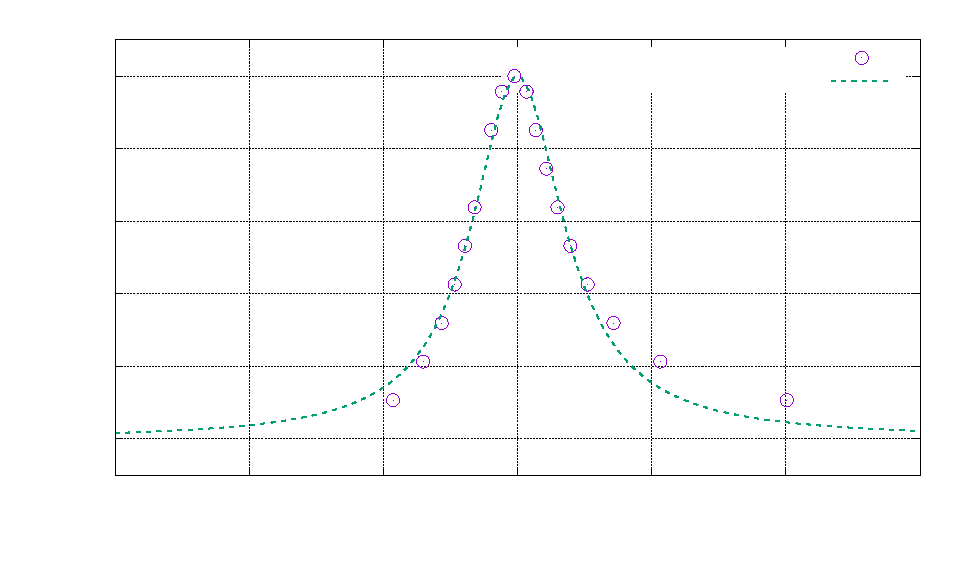
\includegraphics{rezokrivka}}%
    \gplfronttext
  \end{picture}%
\endgroup

		\caption{Redukovaná rezonančná krivka preložená teoretickou závislosťou}
\end{graph}

Hodnoty $y^2(x)$ v grafe 3 boli preložené funkciou podľa teórie tvaru $f(x) = \frac{d^2}{d^2+(x-1/x)^2}$, kde bol parameter
$$d = (0.0417 \pm 0.0011)$$
dopočítaný programom GNUplot. 
%Miera útlmu $d$ bola určená lineárnou interpoláciou nameraných hodnôt najbližších hodnote $y^2$ = 0.5 a využitím vzťahu $d = |x_1 - x_2|$. Nakoľko sa nám počas merania podarilo dostať blízko hodnote $y^2$ = 0.5, chybu merania odhadujeme na 5\%. 

Činiteľ akosti $Q$ bol určený podľa vzťahu (8) a jeho chybu uvažujeme rovnakú ako relatívnu chybu miery útlmu. 

$$ Q = (23.9 \pm 1.2) $$

Rovnako podľa vzťahu (8) určíme aj náhradný sériový odpor obvodu $R_S$, kde chyba je odhadnutá rovnako na 5\%. 

$$ R_S = (58.9\pm 2.9)\: \Omega $$

\newpage
\subsection{Kalibrácia otočného kondenzátora}
Meranie sme vykonávali podľa postupu uvedeného v teórii, kde nami známou kapacitou je $C_1$ = 1100 pF. Rezonančná frekvencia pri tejto kapacite je $f_r = (579.2 \pm 1.1)$ kHz. Namerané hodnoty spolu s vypočítanou kapacitou otočného kondenzátora $C_x$ sú uvedené v tabuľke 7. Tieto hodnoty sú nižšie vynesené do grafu a preložené polynomickou funkciou\footnote{kde $x$ zastupuje premennú $\degree$ vynesenú na x-ovej osi} $g(x)$ tretieho stupňa, ktorá najpresnejšie opisovala body grafu. 

\begin{table}[!htbp]
\captionof{table}{Namerané hodnoty výchyliek na otočnom kondenzátore v závislosti na jeho kapacite $C_x$}
\centering
\begin{tabular}{|l|l|l|l|}
\hline
výchylka [\degree] & $C_1$ [pF] & $C_2$ [pF] & $C_x$ [pF]   \\ \hline
0   & 1100 & 1029.0  & 71.0    \\ \hline
20  & 1100 & 1030.0  & 70.0    \\ \hline
40  & 1100 & 1022.0  & 78.0    \\ \hline
60  & 1100 & 1002.0  & 98.0    \\ \hline
80  & 1100 & 990.0   & 110.0   \\ \hline
100 & 1100 & 863.5 & 236.5 \\ \hline
120 & 1100 & 731.0   & 369.0   \\ \hline
140 & 1100 & 581.5 & 518.5 \\ \hline
160 & 1100 & 362.0   & 738.0   \\ \hline
180 & 1100 & 143.0   & 957.0   \\ \hline
\end{tabular}
\end{table}

\begin{graph}[ht]
		\centering
		% GNUPLOT: LaTeX picture with Postscript
\begingroup
  \makeatletter
  \providecommand\color[2][]{%
    \GenericError{(gnuplot) \space\space\space\@spaces}{%
      Package color not loaded in conjunction with
      terminal option `colourtext'%
    }{See the gnuplot documentation for explanation.%
    }{Either use 'blacktext' in gnuplot or load the package
      color.sty in LaTeX.}%
    \renewcommand\color[2][]{}%
  }%
  \providecommand\includegraphics[2][]{%
    \GenericError{(gnuplot) \space\space\space\@spaces}{%
      Package graphicx or graphics not loaded%
    }{See the gnuplot documentation for explanation.%
    }{The gnuplot epslatex terminal needs graphicx.sty or graphics.sty.}%
    \renewcommand\includegraphics[2][]{}%
  }%
  \providecommand\rotatebox[2]{#2}%
  \@ifundefined{ifGPcolor}{%
    \newif\ifGPcolor
    \GPcolorfalse
  }{}%
  \@ifundefined{ifGPblacktext}{%
    \newif\ifGPblacktext
    \GPblacktexttrue
  }{}%
  % define a \g@addto@macro without @ in the name:
  \let\gplgaddtomacro\g@addto@macro
  % define empty templates for all commands taking text:
  \gdef\gplbacktext{}%
  \gdef\gplfronttext{}%
  \makeatother
  \ifGPblacktext
    % no textcolor at all
    \def\colorrgb#1{}%
    \def\colorgray#1{}%
  \else
    % gray or color?
    \ifGPcolor
      \def\colorrgb#1{\color[rgb]{#1}}%
      \def\colorgray#1{\color[gray]{#1}}%
      \expandafter\def\csname LTw\endcsname{\color{white}}%
      \expandafter\def\csname LTb\endcsname{\color{black}}%
      \expandafter\def\csname LTa\endcsname{\color{black}}%
      \expandafter\def\csname LT0\endcsname{\color[rgb]{1,0,0}}%
      \expandafter\def\csname LT1\endcsname{\color[rgb]{0,1,0}}%
      \expandafter\def\csname LT2\endcsname{\color[rgb]{0,0,1}}%
      \expandafter\def\csname LT3\endcsname{\color[rgb]{1,0,1}}%
      \expandafter\def\csname LT4\endcsname{\color[rgb]{0,1,1}}%
      \expandafter\def\csname LT5\endcsname{\color[rgb]{1,1,0}}%
      \expandafter\def\csname LT6\endcsname{\color[rgb]{0,0,0}}%
      \expandafter\def\csname LT7\endcsname{\color[rgb]{1,0.3,0}}%
      \expandafter\def\csname LT8\endcsname{\color[rgb]{0.5,0.5,0.5}}%
    \else
      % gray
      \def\colorrgb#1{\color{black}}%
      \def\colorgray#1{\color[gray]{#1}}%
      \expandafter\def\csname LTw\endcsname{\color{white}}%
      \expandafter\def\csname LTb\endcsname{\color{black}}%
      \expandafter\def\csname LTa\endcsname{\color{black}}%
      \expandafter\def\csname LT0\endcsname{\color{black}}%
      \expandafter\def\csname LT1\endcsname{\color{black}}%
      \expandafter\def\csname LT2\endcsname{\color{black}}%
      \expandafter\def\csname LT3\endcsname{\color{black}}%
      \expandafter\def\csname LT4\endcsname{\color{black}}%
      \expandafter\def\csname LT5\endcsname{\color{black}}%
      \expandafter\def\csname LT6\endcsname{\color{black}}%
      \expandafter\def\csname LT7\endcsname{\color{black}}%
      \expandafter\def\csname LT8\endcsname{\color{black}}%
    \fi
  \fi
    \setlength{\unitlength}{0.0500bp}%
    \ifx\gptboxheight\undefined%
      \newlength{\gptboxheight}%
      \newlength{\gptboxwidth}%
      \newsavebox{\gptboxtext}%
    \fi%
    \setlength{\fboxrule}{0.5pt}%
    \setlength{\fboxsep}{1pt}%
\begin{picture}(9070.00,5102.00)%
    \gplgaddtomacro\gplbacktext{%
      \csname LTb\endcsname%%
      \put(946,704){\makebox(0,0)[r]{\strut{}$0$}}%
      \csname LTb\endcsname%%
      \put(946,1539){\makebox(0,0)[r]{\strut{}$200$}}%
      \csname LTb\endcsname%%
      \put(946,2375){\makebox(0,0)[r]{\strut{}$400$}}%
      \csname LTb\endcsname%%
      \put(946,3210){\makebox(0,0)[r]{\strut{}$600$}}%
      \csname LTb\endcsname%%
      \put(946,4046){\makebox(0,0)[r]{\strut{}$800$}}%
      \csname LTb\endcsname%%
      \put(946,4881){\makebox(0,0)[r]{\strut{}$1000$}}%
      \csname LTb\endcsname%%
      \put(1278,484){\makebox(0,0){\strut{}$0$}}%
      \csname LTb\endcsname%%
      \put(2077,484){\makebox(0,0){\strut{}$20$}}%
      \csname LTb\endcsname%%
      \put(2877,484){\makebox(0,0){\strut{}$40$}}%
      \csname LTb\endcsname%%
      \put(3676,484){\makebox(0,0){\strut{}$60$}}%
      \csname LTb\endcsname%%
      \put(4476,484){\makebox(0,0){\strut{}$80$}}%
      \csname LTb\endcsname%%
      \put(5275,484){\makebox(0,0){\strut{}$100$}}%
      \csname LTb\endcsname%%
      \put(6075,484){\makebox(0,0){\strut{}$120$}}%
      \csname LTb\endcsname%%
      \put(6874,484){\makebox(0,0){\strut{}$140$}}%
      \csname LTb\endcsname%%
      \put(7674,484){\makebox(0,0){\strut{}$160$}}%
      \csname LTb\endcsname%%
      \put(8473,484){\makebox(0,0){\strut{}$180$}}%
    }%
    \gplgaddtomacro\gplfronttext{%
      \csname LTb\endcsname%%
      \put(198,2792){\rotatebox{-270}{\makebox(0,0){\strut{}$C_x$ [pF]}}}%
      \put(4875,154){\makebox(0,0){\strut{}výchylka [$\degree$]}}%
      \csname LTb\endcsname%%
      \put(3982,4708){\makebox(0,0)[r]{\strut{}aproximačná funkcia $g(x)$}}%
      \csname LTb\endcsname%%
      \put(3982,4488){\makebox(0,0)[r]{\strut{}namerané hodnoty}}%
    }%
    \gplbacktext
    \put(0,0){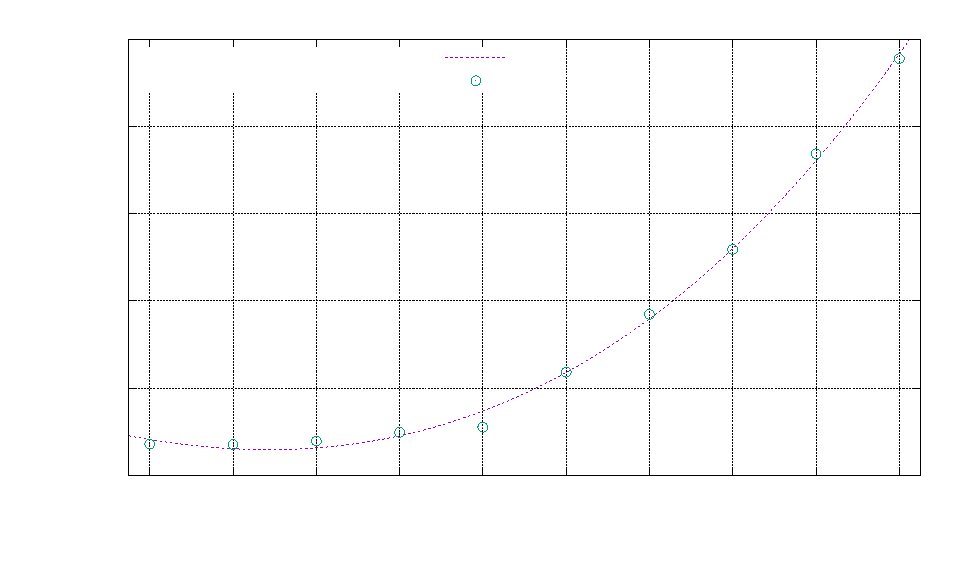
\includegraphics{kalibraciakondenzatora}}%
    \gplfronttext
  \end{picture}%
\endgroup

		\caption{Závislosť kapacity otočného kondenzátoru na výchylke na jeho stupnici}
\end{graph}

$$g(x) = 6.13x^3 + 0.03x^2 - 1.59x + 81.58$$

\newpage
\section{Diskusia výsledkov}
Pri určovaní vlastných kapacít a indukčností oboch cievok a neskôr indukčnosti pri ich sériovom zapojení\footnote{či už pri súhlasnom alebo nesúhlasnom vinutí} sme využili stav rezonancie a teda známe vzťahy pre tento stav obvodu. Rezonančná frekvencia pre rôzne hodnoty zapojeného kondenzátora odpovedala teoretickému vzťahu pre prevrátenú hodnotu druhej mocniny uhlovej frekvencie a to tak, že jej závislosť na kapacite bola vždy lineárna. Meraním sme potvrdili, že reálna cievka disponuje vlastnou kapacitou, ktorá nie je zanedbateľná oproti ideálnej cievke, ktorej vlastnú kapacitu neuvažujeme. K určovaniu rezonančnej frekvencie sme merali rovnaké hodnoty na galvanometri na oboch stranách rezonančnej krivky a priemerom týchto hodnôt sme dopočítavali $f_r$. Tento spôsob bol jednoznačne presnejší, ako meranie maxima, nakoľko nami používaný galvanometer nemal dostatočnú presnosť a hodnoty v príliš veľkom okolí maxima tejto závislosti mali lineárny priebeh. Chybu spôsobenú touto metódou môžeme odhadovať v ráde desatín kHz, no citlivosť použitého galvanometru nebola dostatočná a isté hodnoty sme nedokázali zmerať presne na oboch stranách rezonančnej krivky. 

Vypočítaná hodnota vzájomnej indukčnosti pre dvojicu cievok A,B odpovedá teoretickému vzťahu, kde vypočítané hodnoty sa líšia od nameraných v ráde jednotiek, t.j. tretia platná cifra. Teoretický vzťah môžeme teda považovať za overený. 

Tvar rezonančnej krivky odpovedá teoretickému predpokladu, ale je vidieť, že body nie sú symetrické z oboch strán tak, ako sme predpokladali. Toto je pravdepodobne spôsobené nedostatočným počtom nameraných hodnôt, a teda aj keď je väčšina hodnôt nameraná v symetrických bodoch na tejto krivke, zmeraním viacero hodnôt by sa pravdepodobne vystreďovali a nespôsobili dojem, že meranie je nepresné. Fakt, že namerané hodnoty nie sú symetrické je pravdepodobne spôsobené galvanometrom, nakoľko ukazoval rovnakú výchylku pri príliš veľkom rozmedzí frekvencií. Hodnoty boli preložené teoretickou závislosťou (7) programom GNUplot, ktorý taktiež určil presnosť tohoto fitu metódou najmenších štvorcov. Miera útlmu $d$ bola tiež určená lineárnou interpoláciou nameraných hodnôt najbližších hodnote $y^2$ = 0.5 a využitím vzťahu $d = |x_1 - x_2|$. Takto vypočítaná hodnota parametra d bola v rozmedzí chyby fitu, no nakoľko sa nám počas merania nepodarilo dostať dostatočne blízko k hodnote $y^2$ = 0.5, chyba tohoto výpočtu prevyšovala naše očakávania a ďalej sme uvažovali hodnotu vypočítanú fitom programu GNUplot uvedenú v sekcii 3.4.

Následne sme určili aj hodnotu činiteľa akosti cievky $Q$ a náhradného sériového odporu $R_S$, hodnoty ktorých sú taktiež uvedené v sekcii 3.4.

Otočný kondenzátor sme kalibrovali za rovnakých podmienok ako meranie rezonančnej krivky, t.j. $f_r = (579.2 \pm 1)$ kHz a pevnú kapacitu sme určili ako $C = 1100$ pF, čo bola maximálna hodnota na integrovanom kondenzátore a tú sme zvolili z dôvodu neznalosti kapacity otočného kondenzátora v ani jednom bode výchylky na jeho stupnici. Pri kalibrácii vzniká chyba nepresným určovaním rezonancie pri zmene vnútornej kapacity. Namerané hodnoty boli preložené polynomickou funkciou tretieho stupňa, kde absolútny člen označuje kapacitu pri nulovej výchylke. Tieto hodnoty boli preložené viacerými funkciami podobného tvaru\footnote{napr. exponenciála alebo polynómy iných stupňov} programom GNUplot, no táto vykazovala najmenšiu chybu, t.j. najmenšiu odchýlku od nameraných hodnôt, a teda najpresnejšie určuje závislosť kapacity otočného kondenzátora na výchylke na jeho stupnici. Fakt, že hodnota kapacity pri nulovej výchylke bola vyššia ako tá nasledujúca a teda aj fitovaná funkcia má minimum mimo nulovej výchylky bol pravdepodobne spôsobený systematickou chybou a pre väčšiu presnosť, by bolo nutné ďalšie a to presnejšie meranie.

Chyby všetkých meraní sú prevažne na strane experimentátora. Určovanie kapacity na oboch kondenzátoroch a hlavne nepresná práca s galvanometrom, t.j. nepresné odčítanie hodnôt zo stupníc zapríčinilo väčšinu chýb. 

\section{Záver}
Namerali sme indukčnosti $L$ a vlastné kapacity $C_0$ cievok A,B ako 

$$L_A = (215.0 \pm 1.6)\: {\mu}\text{H},\; C_{0_A} = (56.3 \pm 0.8)\text\: \text{pF}$$
$$L_B = (245.3 \pm 0.7)\: {\mu}\text{H},\; C_{0_B} = (21.7 \pm 1.1)\text\: \text{pF}.$$

Následne sme určili vzájomnú indukčnosť sériovo zapojených cievok z merania závislosti rezonančnej frekvencie na kapacite pri súhlasnom a nesúhlasnom smere vinutia cievok A,B ako

$$ M = (58.8 \pm 3.3) \: {\mu}\text{H},$$

kde jednotlivé indukčnosti pri oboch smeroch vinutia boli
$$ \text{$L_+$ = (571.5 $\pm$ 7.8) $\mu$H, $L_-$ = (336.5 $\pm$ 7.2) $\mu$H}.$$

Namerali sme rezonančnú krivku pre nesúhlasne vinutie cievok A,B a hodnotu $C$ = 200 pF. Maximálna výchylka na galvanometri bola 47. Ako rezonančnú frekvenciu sme použili hodnotu $f_r = (579.2 \pm 1.1)$ kHz a pevnú kapacitu $C = 200$ pF. Namerané hodnoty sme preložili funkciou $f(x) = \frac{d^2}{d^2+(x-1/x)^2}$, ktorá zodpovedá teórii a následne sme určili mieru útlmu ako

$$d = (0.0417 \pm 0.0011)$$

Potom sme tiež určili činiteľ akosti cievky 

$$ Q = (23.9 \pm 1.2) $$
a hodnotu náhradného sériového odporu 

$$ R_S = (58.9\pm 2.9)\:\Omega.$$

Otočný kondenzátor sme kalibrovali za pri rezonančnej frekvencii $f_r = (579.2 \pm 1.1)$ kHz a pevnej kapacite $C = 1100$ pF. Závislosť jeho kapacity na výchylke na jeho stupnici bola nafitovaná funkciou ktorá najpresnejšie opisovala tieto hodnoty je 

$$g(x) = 6.13x^3 + 0.03x^2 - 1.59x + 81.58.$$

\printbibliography

\end{document}
 
\end{document}
